In this chapter of bachelor thesis we will provide a solution of this bachelor thesis problem.
\section{Hardware}
For the start we need device which will be capable of running operating system. There are many various platforms which provide single board computers, we have choosen raspberry platform as most suitable because it is capable of running full linux operating system, have 4 USB slots which will be needed for peripheral devices and foremost there is a pleathora of hardware addons, sensors and boards which works with raspberry models, not to mention availablilty of information how to connect them.
\subsection{Device}
Since we will be building embedded device which will allow us to gather data and send them over to the Internet, it is necessary to choose a single-board computer which provides means for connecting to the Internet either by connectig using built-in hardware or peripheral device. For connecting various sensors \gls{sbc} must provide enough \gls{gpio} pins and support communication protocols commonly used with sensors e.g \gls{i2c}.
After picking the right platform we need to pick model. Newest model on the market from raspberry platform in time of developing this thesis was Raspberry Pi Zero which was not suitable for the needs of this thesis because it does not have any usb ports. It has support for On-the-go USB cables but we need device which supports atleast 2 or 3 usb ports, which we would need to solve by buying USB hubs. We will use Raspberry Pi 2 Model B, as we own one. It has 4 USB ports, 40 GPIO pins and micro SD card slot. This device covers almost all the needs of this thesis. We will need to extend it with WiFi/Bluetooth USB dongle which will enable us to create WiFi access point. In time of writing this thesis Raspberry Foundation released new device Raspberry Pi 3 which is even more suitable for us because it has buitl-in Wireless LAN so no WiFi/Bluetooth USB dongle is neccessary.
\subsection{Operating System}
The most suitable operating system for our needs is Linux based. Concrete distribution of Linux based operating system will be Arch Linux. The main gain of using Arch Linux is it is extremely lightweight distribution with Keep it Simple and Stupid(KISS) principle in mind also it is a rolling release which means it is always up-to-date. Port of Arch Linux distribution is Arch Linux ARM which carries forward the Arch Linux philosophy of simplicity and user-centrism, targeting and accommodating competent Linux users by giving them complete control and responsibility over the system. Instructions are provided to assist in navigating the nuances of installation on the various ARM platforms; however, the system itself will offer little assistance to the user.
Installing and basic configuration of Arch Linux will not be covered in this thesis, as there is enough information available to achieve it. Arch Linux has one of the best documentation online, for those who are not familiar with how to install and configure this particular Linux distribution, follow documentation from Arch Linux website.

\newpage
\section{Configuration} % (fold)
\label{sec:configuration}
In this section we will cover configuration of various applications and system properties to set up the device properly for our needs.
\subsection{Database} % (fold)
\label{sub:database}
For storing information on developing device, it needs to be capable of running database. As it is with linux there, are a lot of databases to choose from and to suit our needs we need to be aware on one fact, and that is where all gathered information will be stored. Raspberry can support very large memory cards, up to 512 gigabytes, and with various read/write speeds, so one could find card which will suit oneself needs.\cite{rpi_sd_cards} In spite of availability of different micro SD cards, everyone has limited read/write cycles after which card become unreliable. Another solution is not to store information on card at all. Typical linux database will create database file to which it stores data, in configurating we could point database to create this file in a special directory. On Linux it is called /tmp\cite{tmp}, this direcory is allocated not on memory card but instead on RAM memory, which would save us need of large and expensive card. It comes with disadvantage, after restart or shutdown of the device, we would not be able to access stored data as RAM memory is votelatile\cite{tmpfs}.
We will use Redis database which has the ability to set the database in RAM memory but it is configurable to save snapshots(copies) to the micro SD card. Redis is an open source, in-memory data structure store, used as database, cache and message broker\cite{redis_doc}. Configuration file for database which runs on our device can be found in resources of this bachelor thesis under name \verb|redis.conf|.
% subsubsection database (end)
\subsection{Wireless Access Point} % (fold)
\label{sub:wireless_access_point}
To automaticly create wireless access point when the device boots up we need several configrations and applications. Firstly the compatibility of device. To create software access point you will need nl80211 compatible wireless device, which support AP operating mode\cite{soft_ap}. Application which will be needed is hostapd, iw and dhcpcd. Configuration file for hostapd can be found in resources under name \verb|hostapd.conf| which needs to be copied into \verb|/etc/hostapd/|, and a systemctl rule, which needs to be copied into \verb|/lib/systemd/system/|. After that reload systemctl dameon, start and enable wifi-ap.service. If you have compliant device it will automatically create wireless Access Point which is defined in hostapd.conf.
% subsubsection wireless_access_point (end)
\subsection{Internet} % (fold)
\label{sub:internet}
As we are using Adafruit FONA 3G Cellular + GPS modem, creating connection to the Internet is possible in different ways. First is using pppd daemon which is capable upon configuration to create ppp0 device which will be used to connect to the internet. Configuration files for ppp can be found in resources under folred in \verb|ppp| folder. Another approach is with wvdial, which configuration can also be found in repository. At last FONA 3G is supported by QMI modem protocol. For dialing with qmi one needs to install libqmi and net-tools packages. You will need to know to which apn you need to connect from your mobile internet service provider. After that replace APN in qmi-network.conf from config folder at GitHub, copy it to \verb|/etc/|. From script folder found in thesis repository copy a helper script, and then simple \verb|qmi_setup.sh start| starts the connection to the internet. If your SIM card is PIN locked you will need to unlock it manually trough AT command or with help from \verb|mmcli| command.
% subsubsection internet (end)
% subsection configuration (end)
\newpage
\section{Peripherals} % (fold)
\label{sec:peripherals}
For providing proof of concept device which is capable of gathering information from various sources we will connect to the device numerous peripherals which will generate information. Peripherals will be described in upcoming subsections and configuration instructions will be provided. We believe that connecting this peripherals is such trivial that it does not need to be explained to the reader, if however someone would not have sufficient knowledge of how to connect these to the raspberry pi we suggest to find some guide on the internet for correct connections to be made. Overview of peripherals connected to device is provided below in Table \ref{tab:tab2}.
\begin{table}[H]
 \begin{center}
   \begin{tabular}{l l}
   Peripheral device & Connected by\\
   \hline
   	Wireless/Bluetooth dongle & USB\\
	Adafruit 10-DOF & \gls{i2c} bus\\
	Adafruit FONA 3G Cellular + GPS & USB(creates 4 virtual serial ports)\\
	ELM327 Compatilbe device & USB\\
   \hline
   \end{tabular}
 \end{center}
 \caption{Peripheral devices connected to Raspberry Pi}
 \label{tab:tab2}
\end{table}
\subsection{Adafruit 10-DOF} % (fold)
\label{sub:adafruit_10_dof}
As for configuration you will need packages \verb|i2c-tools| and \verb|lm_sensors|, then get config config.txt from thesis reposirtory and copy it to /boot/config.txt, enable mondules \verb|i2c-dev, i2c-bcm2708| in \verb|/etc/modules-load.d/raspberrypi.conf|. That is it, now with command \verb|i2cdetect -y 0| it should work, if not follow troubleshoot documentation on raspberry pi on archlinux wiki\cite{rpi_wiki}.
% subsubsection adafruit_10_dof (end)
\subsection{Adafruit FONA 3G Cellular + GPS} % (fold)
\label{sub:adafruit_fona_3g_cellular_gps_}
 As for configuration there are multiple ways how to connect to the internet, send SMS and make voice calls, all of them boils down to using right AT commands through serial console which is automatically created by the kernel.After connecting modem through usb to the raspberry, kernel will create 4 serial ports(debug,nmea,serial,modem). After starting gps chip with correct command \verb|at+cgps=1| at serial port nmea will start to push gps data on nmea port at 115200 baud rate.\cite{at_doc}
% subsubsection adafruit_fona_3g_cellular_gps_ (end)
% subsection peripherals (end)
\subsection{OBD-II connection} % (fold)
\label{sub:obd_ii_connection}
Connection to \gls{obd} port is possible by various devices which interface \gls{obd} to other standards such as USB, \gls{i2c}, SPI, CAN. To be able to connect to the \gls{obd} port by various devices not only by Raspberry Pi, we have choosen ELM-USB.
% subsubsection connection (end)
\subsubsection{Configuration} % (fold)
\label{ssub:configuration}
To be able successfuly connect to the OBD-II port of the vehicle it is necessary to select proper protocol to communicate. There are two possibilities how to do that. Firtsly ELM-USB device can be configured to use Automatic protocol detection or specificaly instructed to use defined protocol. Command for this configuration is \verb|AT SP X|\cite{at_cmd} where x is one of values defined at Table~\ref{tab:tab3}
\begin{table}[H]
 \begin{center}
   \begin{tabular}{l l}
   X & Communication protocol\\
   \hline
	0 & Automatic protocol detection \\
	1 & SAE J1850 PWM (41.6 kbaud) \\
	2 & SAE J1850 VPW (10.4 kbaud) \\
	3 & ISO 9141-2 (5 baud init, 10.4 kbaud) \\
	4 & ISO 14230-4 KWP (5 baud init, 10.4 kbaud) \\
	5 & ISO 14230-4 KWP (fast init, 10.4 kbaud) \\
	6 & ISO 15765-4 CAN (11 bit ID, 500 kbaud) \\
	7 & ISO 15765-4 CAN (29 bit ID, 500 kbaud) \\
	8 & ISO 15765-4 CAN (11 bit ID, 250 kbaud) - used mainly on utility vehicles and Volvo \\
	9 & ISO 15765-4 CAN (29 bit ID, 250 kbaud) - used mainly on utility vehicles and Volvo \\
   \hline
   \end{tabular}
 \end{center}
 \caption{Communication protocols of ELM-USB}
 \label{tab:tab3}
\end{table}
% subsubsection configuration (end) 
% subsection obd_ii_connection (end)
\section{Software} % (fold)
\label{sec:software}
\subsection{Problem abstraction} % (fold)
\label{sub:problem_abstraction}
To solve given task, lets firts look at data gathering and what can be done to optimize proccess of collecting infromation from often very different sources. For correct conclusion to be made, we need to abstract the meaning of car connection as merely only as one of infromation sources. To solve how to easily interconnect different input sources(information producing) to even more different output sinks(information sending), a framework was developed. A data applicaton module which will provide easy connecting of different sources with data producing modules to any data accepting modules. So to begin lets define some construction blocks of this framework so we can easily build a suitable application.
% subsection problem_abstraction (end)
\subsection{Data-Logger framework} % (fold)
Data-Logger framework is a stand alone application module which can be incorporated in any Node.js application. Main principle of the framework can be descripted by pipes and filters design pattern. In pipes and filters design pattern a pipeline consists of chain of processing elements arranged in a way where output of each element is the input of the next, same as physical pipes together to form a pipeline. In the framework the information which is passed along is data collected by source modules from devices which generate data e.g. sensors. Pipes and filters design can be viewed as form of functional programming, using streams as data objects. They could even be seen as a particular form of monad for I/O\cite{monad_pipe}. Main goal of this framework is to provide easy way how to setup communication between various inputs(sensoric data, IoT devices, cars, etc.) and outputs(database, application, server, cloud, etc). Framework is structured by main app, modules and routes. Their relations are as shown in Figure \ref{fig:entity_pc}.
\begin{figure}[H]
\begin{center}
\captionsetup{font=small}
\includegraphics[scale=0.7]{pics/entity_bc.png}
\caption{Entity diagram of Data-Logger framework}
\label{fig:entity_pc}
\end{center}
\end{figure}
 Modules are stand alone application modules which are written to obtain,modify, or send data to various devices or services. Pipes and filters design is applied when connecting modules together. How are modules connected is defined by routes. which are an interface for configuring which module will be streaming data to which. Data-Logger is configurable through internal function and by file which serves for storing configurations of each model and route. To help understand dataflow of the Data-Logger we provide diagram in Figure~\ref{fig:dataflow}.
 \begin{figure}[H]
\begin{center}
\captionsetup{font=small}
\includegraphics[scale=0.6]{pics/data_flow_bc.png}
\caption{Dataflow of Data-Logger framework}
\label{fig:dataflow}
\end{center}
\end{figure}
\subsubsection{Module}
\label{ssub:module}
Application Module is basic structure for every element in Data-Logger. It is an encapsulating class for every information creating or sending application. By this it is possible for framework to objectify every application, no matter how much they would be different, and extract data from generating one or send data to to accepting one. With this feature we will be able to get data from OBD port of the car system the same way as from accelometer present at Adafruit 10 DOF sensoric board. This is achieved by writing specific applications to parse/get data from the source, which are then run under Data-Logger. Every module can be generating data, or accepting data and acting upon it. For module to be generating or accepting one, module must be implemented by the same interface so it can be easily handled by Data-Logger, otherwise for every application connected to Data-Logger there would had to be specific functions to run to obtain or accept data. Configurating modules are easy as from framework we can pass settings for every module separatly, either from application or much easier from a main configuration file. This configuration file has a specific block of configruation settings for every module present in current implementation of Data-Logger. To provide better description of what data-logger module consists we provide activity diagram in Figure~\ref{fig:activity}
\begin{figure}[H]
\begin{center}
\captionsetup{font=small}
\includegraphics[scale=0.6]{pics/logic_bc.png}
\caption{Activity of Data-Logger module}
\label{fig:activity}
\end{center}
\end{figure}
\subsubsection{Route} % (fold)
\label{ssub:route}
Route is another basic structure how to define a dataflow from or to every module. Routes are defined with simple principle in mind: you define source and then every possible sink to which data have to be sent. By this configuration Data-Logger will start sending or recieving data from modules depending on which side of the equation they are. If the module is generating data, framework will use specific general interface to gather data provided by the module and then distribute it to every sink defined by the route again by using general interface to sending data to module. With this principle one can define a very detailed dataflow. If we would scale this framework, say we would have 10 sensors producing same data but they would need different modules to be handled, it would become soon tedious to write routes based only on unique identification matching of modules. So for every module there is a specific setting to be set, a type, by which we can more easily define routes, e.g. defined route as \verb|accelerometer -> database| and from now on, every data produced by module which has type set to acceloremeter will be routed to every module which has database set as type. Activity diagram of Data-Logger routes is shown in Figure~\ref{fig:act}. 
\begin{figure}[H]
\begin{center}
\captionsetup{font=small}
\includegraphics[scale=0.6]{pics/route_bc.png}
\caption{Activity of Data-Logger routes}
\label{fig:act}
\end{center}
\end{figure}
% subsubsection route (end)
\label{sub:data_logger_framework}
% subsection data_logger_framework (end)
\subsection{Data-Logger low-level modules}

In this section of bachelor thesis we will desciribe modules which were developed in order to help complete the assignment. Low-level modules are modules which does not implement any logic or process data in any way. They are developed for simple reason of data gathering or sending. If they recieve messages, low-level module does not alter contents of messages, just sends them to the destination determined by the module.
\subsubsection{Blank module} % (fold)
\label{ssub:blank_module}
During developing modules for this bachelor thesis, a blank module was created which has all the necessary functions, interface to make more easier creation of new modules. Code is commented to provide viable information what is expected from different functions in case their name would not be clarifying enough. Blank module combines source and sink functionality together but they do not need to be used both.
% subsubsection blank_module (end)
\subsubsection{Time module} % (fold)
\label{ssub:time_module}
This is rather simple module which will be used to beta test others modules. Advantage of having this module is not being dependent on any hardware. In periodic intervals defined by sample rate, current time as data is provided.
% subsubsection time_module (end)
\subsubsection{Accelerometer module} % (fold)
This module is dependent on Adafruit 10 DOF sensor board and will utilize onboard LSM303 accelerometer sensor, communicating over I2C protocol. Module will emit proper acceleration in 3 axis, maximum acceleration +- 16g in each direction, sample rate will be configurable. LSM303 accelerometer sensor supports various settings as which axis acceleration is registered, how fast are these values checked, the constants for these settings are implemented, but any benefit was not found of selecting only one axis or sampling at lower rate, so defaults are every axis is registered, and sampled as fast as it can be for accident checking module.
% subsubsection accelerometer_module (end)
\label{ssub:accelerometer_module}
\subsubsection{GPS module} % (fold)
\label{ssub:gps_module}
GPS module as name suggests will parse nmea sentences from FONA 3g modem which has built-in GPS chip. AS for this module there is not much to be configured, because modem emits nmea sentences at 115200 baud rate as fast as it can, meaning every second, only thing found which could be configured is to switch output port for nmea sentences from nmea to serial, but then sending SMS and calling would not be possible, so it is not a feasible setting.
% subsubsection gps_module (end)
% subsubsection accident_module (end)
\subsubsection{SMS module} % (fold)
\label{ssub:sms_module}
This module is a sms message sending module, but it is not designed for general use. Message relays on incoming data to be structured correctly from accident module and send 3 SMS messages with information about driver, GPS position and maximum g-force registered by the accelerometer. Module requires modem to be pin unlocked otherwise SMS sending will fail. Sending SMS message with \verb|AT+CGMS| command requires string to be sent with a maximal size of 150 characters and ended with \verb|^Z| special character. After message is sent, module repsonds with OK and number of total SMS messages sent by the module.
% subsubsection sms_module (end)
\subsubsection{OBD-II module} % (fold)
By far the most challenging module in this thesis. Module connects with help of ELM327 compatible device to the OBD-II port and selects automatic protocol. Problem with automatic protocol selection is protocols have different initializing response, the module needed to be adapted to this discovery, to be working with older and newer cars, we successfuly tested this module on 5 different cars in make and model, but we can not rule out the possibility of OBD module not working with specific model and make of car, because there are multiple protocols present and their specification is not publicly available for free. After successful initialization, OBD-II module will poll the connected car for supported commands which creates a polling loop out of commands which are supported for that particular vehicle and periodicaly queries the data. One must be vary of this one limitation, and that is older cars have older protocols which have slow rate of sending data, and therefore sample rate of this module should be considered to be calculated correctly, otherwise buffer overflow might occur. Module implements simple buffer overflow logic, when length of PID commands queue becomes more than treshold OBD module will not add more commands to queue until the length lowers than treshold. Module emits data for every queried command separately as in some cases gathering information from every supported command would simply took too long time to collect.
\label{ssub:obd_ii_module}

% subsubsection obd_ii_module (end)
\subsubsection{RabbitMQ module} % (fold)
\label{ssub:rabbitmq_module}
RabbitMQ module is primary module for getting data from Rapsberry to server or cloud service. Module client connects to rabbitMQ server, after which it creates queues on the server based on message header id. Implication is that on server we will have queues for every module uploading data. Server then can process this queues separately with data processing applications and have various services to evaulate data and/or act upon it. In testing this module average speed of delivering messages was 500 messages in one second, this rate is based on how big information is being passed onto the server, so for example data from bulk module might have less throughput than accelerometer data. Connection settings can be altered in configuration file.
% subsubsection rabbitmq_module (end)
\subsubsection{Redis module} % (fold)
\label{ssub:redis_module}
Redis module is database module for storing data in Redis database. Redis stores data in mapping keys to values. For correct work module implements counters for every data source which wants to store data in database. Module stores whole given messages in hash keys. Key is composed from message header id and counter which is incremented by every message stored. As not to store counters in modules, counter current value is stored by message header id key. By configuring database snapshoting, redis database is able to recreate data structure from previous sessions, and continue where application left, with correct counters so data would not be accidentaly overriden. Database is password protected which is set by configuration file.
% subsubsection redis_module (end)
\subsubsection{IFTTT module} % (fold)
\label{ssub:ifttt_module}
IFTTT module is a support module for communicating with web service called Maker. With this service one can create different trigger events for data which arrives to the event and connect them to various other web services as GMail, Facebook, Instagram, etc. Data format is limited as Maker channel supports JSON format with only 3 keys, namely \verb|value1,value2,vaule3|, so complicated data structures are not suited for this module. Values of this 3 keys can be any string, with this in mind, the limitation could be circumvented for example with CSV format of data, which can be automatically parsed by for example google drive spreadsheet application. Fair to say is that this service is free of charge and provides with possibilities to connect data generated with vast number of popular web services.
% subsubsection ifttt_module (end)
\subsubsection{Console module} % (fold)
\label{ssub:console_module}
Very simple module which provides structured module for console logging data to show what information is passed into module. This module was primarily used for developing purposes same as time module. This module will probably not be used in production enviroment but is very handy for debuggind purposes, when modules do not cooperate in expected way. Console header can be set only to show configuration capabilities in early stages of development.
\subsection{Data-Logger high-level modules}

High-level modules are modules that implement logic or process data. They are developed for data manipulation, grouping or analyzing, mainly by connecting low-level modules to them and analyzing data from different sources.
\subsubsection{RPM advisor module} % (fold)
\label{ssub:rpm_module}
RPM module is a module which listens for data from OBD-II module and evaluates only RPM(Revolutions per minute) data from car. Purpose of this module is to simulate modern cars which often provides gearshift indicator together with information when to shift. In configuration file can be find two values, downShiftTreshold and upShiftTreshold. When RPMs drops under downShiftTreshold treshold, module will generate data to indicate to shift gears, similiar action happens with upShiftTreshold, but instead dropping RPMs, module triggers when revolutions are higher then treshold as can be seen in Figure~\ref{fig:rmp_pic}
\begin{figure}[H]
\begin{center}
\captionsetup{font=small}
\includegraphics[scale=0.6]{pics/RPM_bc.png}
\caption{Activity diagram of RMP advisor module}
\label{fig:rmp_pic}
\end{center}
\end{figure}
This module have also configured IFTTT event. This event triggers a notification on mobile device which has IFTTT application installed. In the screenshots below shown as Figure~\ref{fig:mobile_screen} we can see what it looks like.
\begin{figure}[H]
\begin{center}
\captionsetup{font=small}
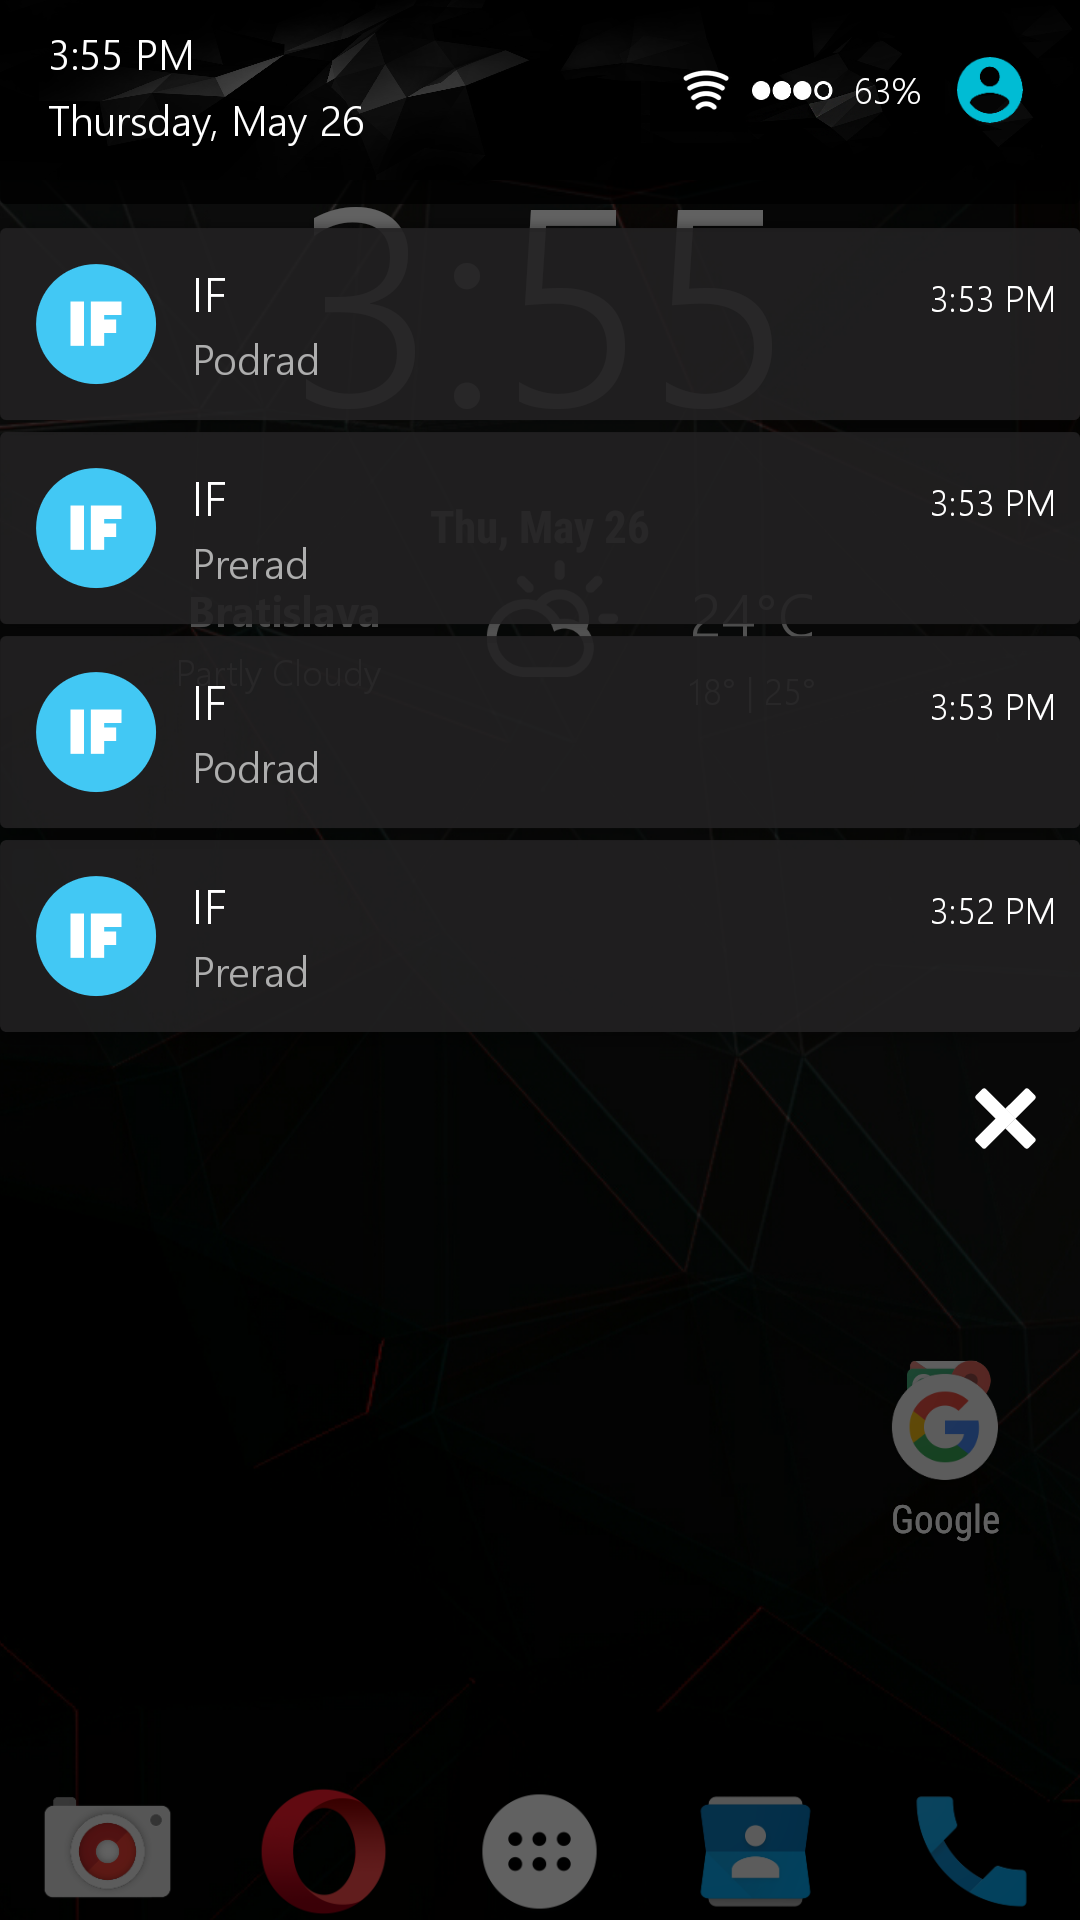
\includegraphics[scale=0.2]{pics/mobil_screen.png}
\caption{Screenshot of RPM advisor notifications}
\label{fig:mobile_screen}
\end{center}
\end{figure}
% subsubsection rpm_module (end)
% subsubsection console_module (end)
\subsubsection{Bulk module} % (fold)
Bulk module is module primarily used for grouping outputs from multiple modules into one big message. Reason for grouping messages is sending data over Internet rather in burst mode than constant stream. In bulk module settings user can choose time interval and size treshold for sending data. Whichever happens first triggers sending the message.
\label{ssub:bulk_module}
% subsubsection bulk_module (end)
\subsubsection{Accident module} % (fold)
\label{ssub:accident_module}
This module will be both accepting input data and creating new information for other modules. Electronic crash sensors found in new cars are accelometers. They are used to determine exactly when the airbag should be deployed to prevent injury to a driver or passenger. When an impact occurs, it results in vehicle deceleration, which is sensed by the accelerometer. This change is monitored by electronic control unit, which sends a signal to trigger the airbag. Not to rely on car accelerometer sensors the application will be polling LSM303 accelerometer sensor attached to the device. Problem with car accelerometer sensors is missing common interface to communicate with airbag/ECU system. If it is even possible then every car manafacturer has proprietary system in place, which would result in buying different specifications for every make, maybe even model. As we are not physicists we could not successfully determine at which value from accelerometer is right to register accident. But we created this module that in settings can be found treshold value which says that if accelerometer module registers acceleration over treshold, accident module will be trigered and will compose a SOS message to be sent to emergency dispatch centre as shown in Figure~\ref{fig:acc_bc} This message will be composed of latest GPS positon, maximal g-forces registred and medical information about driver. Medical information about driver, or in other words custom message is also configurable through settings.
\begin{figure}[H]
\begin{center}
\captionsetup{font=small}
\includegraphics[scale=0.6]{pics/accident_bc.png}
\caption{Activity diagram of Accident module}
\label{fig:acc_bc}
\end{center}
\end{figure}
% subsection data_logger_modules (end)
\subsection{Data-Logger routes} % (fold)
\label{sub:data_logger_routes}
Data-Logger routes are designed for interconnecting data streams from modules. These routes are designed so they would fullifil given assignment. Exact definiton how routes are set can be found in a configuration file. Main benefit of having these routes in one place and so easy configurable is that you can change complete outcome of the application by changing routes and redefinig them to suit your needs. All defined routes for our Data-Logger solution are provided in Table~\ref{tab:tab6}
\begin{table}[H]
 \begin{center}
   \begin{tabular}{l l}
   Source Module ID or type & Destination module IDs or types\\
   \hline
   	obd & rpm, bulk, redisModule\\
    rpm & ifttt\\
    acc & bulk,accident, redisModule\\
    gps & bulk, accident, redisModule\\
    accident & sms\\
    bulk & rabbitmqModule\\
   \hline
   \end{tabular}
 \end{center}
 \caption{Routes defined for Data-Logger of this thesis}
 \label{tab:tab6}
\end{table}
% subsection data_logger_routes (end)
\subsection{Main application} % (fold)
\label{sub:main_application}
Main application is the main part of code which is directily run by Node.js. Architecture of the main application can be described as loosely coupled system, where main application has and makes use of little to no knowledge of the Data-Logger framework. This allows for extensibility in design, a new module for framework implementing blank module interface can be written to replace a current modules without requiring a change of the main application. The new and old modules can be interchanged freely. Whole main application can be divided by features. In this section of this work every feature is described separately to provide more detail.
\subsubsection{Web Server} % (fold)
\label{ssub:web_server}
To provide web application for the user to be able to configure Data-Logger framework, server had to be created. This server works at port 8000 at localhost as to not confuse the server address with regular website. To connect to server, you have to be connected to the raspberry, either via LAN cable or to the wireless AP created automaticaly by the raspberry device. Password for this access point can be found in configuration file of hostapd in resources under name \verb|hostapd.conf|. Server supports websockets to communicate real-time with Web Application, also for configuring module settings.
% subsubsection web_server (end)
\subsubsection{Web Socket} % (fold)
\label{ssub:web_socket}
For web application to display real time data produced by Data-Logger modules websockets are used. For every module which produces data, main application will emit the information over websocket to every connected client. After connection client automatically starts listening for emitted info and display it accordingly. Through websockets it is possible to send new configuration to the server. Validating new configuration is burden for the web application as websockets assumes that configuration is written correctly.
% subsubsection web_socket (end)
\subsubsection{Web Application} % (fold)
\label{ssub:web_application}
Once you are connected to the raspberry, open your favorite web browser and enter default ip address of raspberry device which, if you did not change original configuration is \verb|http://10.1.1.100:8000/|. After opening web application you will be presented with simple layout. At the top of website, navigation bar is displayed for switching between configurations of each module, configuration of routes and main page. On main page you will be provided with real time data generated by the modules. In module pages current configuration is displayed which is queried by get request to the server. Server then reads current configuration from file, parsing it and sending it back to web applicaton. Module settings can be changed by clickng configure button. A form will be presented which will allow to add,delete and configure settings. After finishing there is the possibility to either confirm or cancel new settings. When confirmed, web application will check for syntax correctness. Websocket will be used for sendning new configuration to the main application. After getting data to the server it's passed to the Data-Logger framework to update changes to the running Data-Logger and write them to the configuration file for changes to be persistent.
% subsubsection web_application (end)
% subsubsection main_application (end)
% subsection software (end)